\documentclass[12pt, a4paper]{article}
\usepackage{amsmath}
\usepackage{amsfonts}
\usepackage{amsthm}
\usepackage{mathtools}
\newtheorem{theorem}{Theorem}[section]
\newtheorem{definition}{Definition}[section]
\numberwithin{equation}{section}
\usepackage{pgfplots}
\pgfplotsset{width=10cm,compat=1.9}
\graphicspath{ {img/} }
\DeclareGraphicsExtensions{.png}

\title{Convolutional Neural Networks}
\author{Kristian Wichmann}

\begin{document}
\maketitle

\section{Mathematical convolution}
In mathematics, the \textit{convolution} of two functions $f$ and $g$ is defined as:
\begin{equation}
(f*g)(t)=\int_{-\infty}^\infty f(\tau)g(t-\tau)\ d\tau
\end{equation}
By a change of variables $\sigma=t-\tau$, we have $\tau=t-\sigma$, and therefore $d\tau/d\sigma=-1$. Therefore:
\begin{equation}
(f*g)(t)=\int_\infty^{-\infty}f(t-\sigma)g(\sigma)(-d\sigma)=\int_{-\infty}^\infty f(t-\sigma)g(\sigma)\ d\sigma=(g*f)(t)
\end{equation}

\subsection{Discrete convolution}
If $f$ and $g$ are only defined on evenly spaced lattice points the integral in the convolution turns into a sum. Without loss of generality, we can assume these lattice points to be the integers:
\begin{equation}
(f*g)(x)=\sum_{\Delta x\in\mathbb{Z}}f(\Delta x)g(x-\Delta x),\quad x\in\mathbb{Z}
\end{equation}
We will only consider the case, where both $f$ and $g$ is non-zero for most values. Which means that the infinite sum will always be finite in practice, at least in this application.

In two dimensions, the functions are defined on $\mathbb{Z}\times\mathbb{Z}$ instead, and $x,\Delta x\in\mathbb{Z}\times\mathbb{Z}$ as well:
\begin{equation}
(f*g)(x)=\sum_{\Delta x\in\mathbb{Z}\times\mathbb{Z}}f(\Delta x)g(x-\Delta x),\quad x\in\mathbb{Z}\times\mathbb{Z}
\label{2d_convolution}
\end{equation}

\subsection{Discrete convolution for finite lattices}
Now, consider the case where both $f$ and $g$ only take on non-zero values in a rectangular area. Specifically, let $f$ only be non-zero for $\{-F,-F+1,\ldots,-1,0,1,\ldots,F\}\times\{-F,-F+1,\ldots,-1,0,1,\ldots,F\}\times$ and $g$ only non-zero for $\{0,1,\ldots,W-1\}\times\{0,1,\ldots,H-1\}\times$. Then equation \ref{2d_convolution} becomes:
\begin{equation}
(f*g)(i,j)=\sum_{m=-F}^F\sum_{n=-F}^F f(m,n)g(i-m,j-n)
\label{finite_2d_convolution}
\end{equation}
Here, we have explicitly written out the indices of the input.

\subsection{Cross-correlation}
Looking at equation \ref{finite_2d_convolution}, notice that $m$ and $n$ are subtracted in the $g$ arguments. It turns out, that for convenience (and to follow convention), we'd like these to be added instead. The resulating quantity is called the \textit{cross-correlation}:
\begin{equation}
(f\otimes g)(i,j)=\sum_{m=-F}^F\sum_{n=-F}^F f(m,n)g(i+m,j+n)
\label{cross_correlation}
\end{equation}
This means, that we can view this as a convolution where the values of $f$ are mirrored in both directions (or rotated 180 degrees - same thing). So:
\begin{equation}
(f\otimes g)=(f^-*g),\quad f^-(i,j)=f(-i,-j)
\end{equation}

\section{Filters and convolutions}

\subsection{Example: Edge detection}

\begin{figure}
\centering
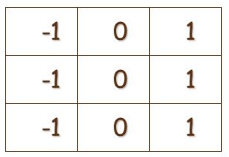
\includegraphics[width=0.4\textwidth]{horizontal_edge}
\caption{A filter for horizontal edge detection.}
\label{fig:horizontal_edge}
\end{figure}

Say we have a black and white image represented in an array of pixel values. If we want to detect horizontal edges, we can think of this as determining the pixel value gradient in the $x$ direction. This should be done all over the picture. One such way to do this, is to look at the immediate neighborhood of pixel value around each point in the picture, i.e. nine pixels in total. Then multiply them by the numbers in the $3\times 3$ matrix shown in figure \ref{fig:horizontal_edge}, and add up all nine values as shown by figure \ref{fig:convolutional_filter}. This will be an approximation to the gradient in the $x$ direction (the opposite of figure \ref{fig:horizontal_edge}, though) in the vicinity of the middle pixel as desired (or at least proportinal to it). In figure \ref{fig:convolutional_filter} we see that overall, the gradient is to the right, which the negative result reflects.

\begin{figure}
\centering
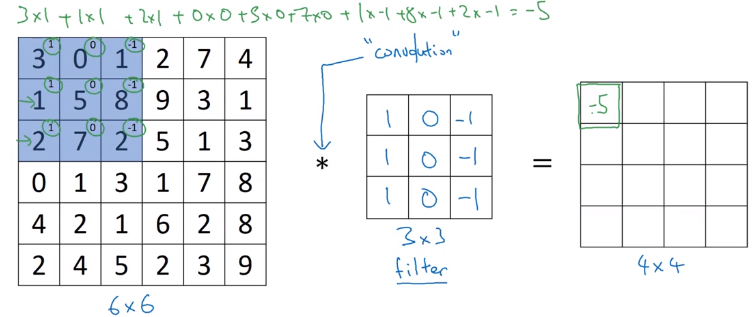
\includegraphics[width=\textwidth]{convolutional_filter}
\caption{How convolution works.}
\label{fig:convolutional_filter}
\end{figure}

For a $n\times n$ image, we can repeat this process for $(n-2)\times(n-2)$ sets of $3\times 3$ blocks of pixels. So the results of the convolution can be represented as an image slightly smaller than the original. Below we will look at how we can avoid this shrinkage.

\subsection{General filter}
There is nothing special about the number in the filters we've used in the edge detection example above. In fact, a central idea in convolutional neural networks is for the algorithm to learn the values of a filter. These are also sometimes known as \textit{kernels}.

Also filter need not be $3\times 3$. It can have any size, but square with an uneven number of pixels on each side is the most common.

\subsection{Padding}
The procedure above is the same as the cross-correlation described in equation \ref{cross_correlation} with $f$ being the filter and $g$ being the image. But here, we will simply refer to it a convolution. But there will be some of the non-zero . Instead we can think of the remaining, infinite number of values to be zero. And we then only consider the non-trivial output window.

But this actually gives ud a way to avoid the image size shrinkage inherent to filtering: As we saw above, a $n\times n$ image convoluted by an $f\times f$ filter results in an output of size $(n-f+1)\times(n-f+1)$. However, if we pad the input image with zeros in all directions, we can avoid this problem. If we pad by $p$ zeros in all four directions, we now get a new input size of $(n+2p)\times(n+2p)$. We want an output size of $(n-f+1)\times(n-f+1)$ as before:
\begin{equation}
n+2p=n-f+1\Leftrightarrow p=\frac{f-1}{2}
\end{equation}
So we will need a margin of zeroes of thickness $p=(f-1)/2$ to keep the image size. Here we see why $f$ is usually chosen to be odd.

Having no padding is sometimes knows as a \textit{valid} convolution, while padding to preserve image size as described above is called a \textit{same} convolution.

\subsection{Stride}
So far, we've used a \textit{stride} $s$ of 1, which means that every time we've moved the convolutional filter we've moved it a single pixel. But we might as well have moved it two or more pixels (both directions). The amount moved is the stride.

With stride 1, an input size of $n\times n$ with padding $p$ results in an output of $n+2p-f+1$ as shown above. But when we move $s$ pixels at a time, we have to divide by $s$ for an output size of:
\begin{equation}
\frac{n+2p-f}{s}+1
\end{equation}
Now, what happens if the fraction is not an integer? In that case, we miss the "last" point. So we have to take the integer part, i.e. rounding down:
\begin{equation}
\left\lfloor\frac{n+2p-f}{s}\right\rfloor+1
\end{equation}

\section{Layers in convolutional networks}

\subsection{Convolution of multiple channels}
An image is typically not black and white, but has colors. This means that is has three \textit{channels}, namely red, green, and blue, or RGB. This is notated as a seperate dimension. So such a color image of height 300, width 200 would have dimensions $200\times 200\times 3$.

Similarly, if we want to apply a filter for convolution, there must be a matrix of numbers for each channel. So a 5 by 5 pixel filter on a RGB image would have dimensions $5\times 5\times 3$. Because the convoutional sum is now over three dimensions, the output will be two-dimensional. For instance if a $100\times 100\times 3$ image is convoluted by a $5\times 5\times 3$ filter, we would get a $96\times 96$ "image" as output (remember the $n-f+1$ formula).

Now, image we have $n$ such filters. Then we may collect all the two dimensional outputs into a new three dimensional object. For instance, if we had 10 filters in the example above, we would end up with a $96\times 96\times 10$ object as output. I.e. the number of filters in one layer is equal to the number of channels in the next.

\subsection{A convolutional layer}
The above outlines most of the elements of a convolutional layer, but we still need two key elements: bias and activation function.

The bias is a number that's added after the convolution summation over the "filter cube" is done. So it is a parameter specific to each filter. The (non-linear) activation function is then applied to the result. The result is the "pixel value" in the output "image".

So the convolutional layer $l$ in a neural network has the following parameters:
\begin{itemize}
\item $f^{[l]}$ - The size of the square filter for a single channel. So $f^{[l]}\times f^{[l]}$.
\item $p^{[l]}$ - The amount of padding that is applied to images before convolution.
\item $s^{[l]}$ - The stride used (only in the two image dimensions).
\end{itemize}
Input and output are tensors (generalized matrices):
\begin{itemize}
\item Input has dimension $n_H^{[l-1]}\times n_W^{[l-1]}\times n_c^{[l-1]}$, where $l-1$ is the previous layer. Subscripts are for height, width, and number of channels, respectively.
\item Similarly, output has dimensions $n_H^{[l]}\times n_W^{[l]}\times n_c^{[l]}$.
\end{itemize}
As discussed above, the relationship between the height and width of the layers is:
\begin{equation}
n_H^{[l]}=\left\lfloor\frac{n_H^{[l-1]}+2p^{[l]}-f^{[l]}}{s^{[l]}}\right\rfloor+1,\quad n_W^{[l]}=\left\lfloor\frac{n_W^{[l-1]}+2p^{[l]}-f^{[l]}}{s^{[l]}}\right\rfloor+1
\end{equation}
The layer contains $n_c^{[l]}$ filters, corresponding to the number of output channels. Each filter has a set of weights of dimension $f^{[l]}\times f^{[l]}\times n_c^{[l-1]}$, since the depth must be equal to the number of channels the last layer outputs. And an additional bias term.

The resulting activations outputs $a^{[l]}$ have dimension $n_H^{[l]}\times n_W^{[l]}\times n_c^{[l]}$ as mentioned above. But this is for a single input image. If we have $m$ data samples, then the collective output $A^{[l]}$ is of dimension $m\times n_H^{[l]}\times n_W^{[l]}\times n_c^{[l]}$.

Similarly, we can collect all the non-bias filter weights in one object of dimension $f^{[l]}\times f^{[l]}\times n_c^{[l-1]}\times n_c^{[l]}$. The biases will be a vector of dimension $n_c^{[l]}$, though we will sometimes consider it to have dimension $1\times 1\times 1\times n_c^{[l]}$.

\subsection{Example of convolutional network}
As an example, let's say out input is $39\times 39$ pixel RGB images. I.e. the inputs to the network are $39\times 39\times 3$.

The first convolutional layer has 10 filters of size $3\times 3$. Stride is 1, and there's no padding. Meaning that the output is $37\times 37\times 10$.

The second convolutional layer has 20 filters of size $5\times 5$. This time stride is 2, but there's still no padding. The output then is $17\times 17\times 20$.

A third and final convolutional layer with 40 filter, again with size $5\times 5$, stride is 2, and no padding. Then the output is $7\times 7\times 40$.

Now, this means we have $7\cdot 7\cdot 40=1960$ features to describe the initial image. Usually this is then fed into one or more fully connected layers to perform classification, or whatever is the goal of the task at hand.

\subsection{Pooling layers}
There's still one commonly used type of layer we haven't touched upon, namely \textit{pooling layers}. These are added to speed up computations by throwing away information strategically.

\subsubsection{Max pooling layers}
Consider the input image shown to the left in figure \ref{fig:max_pooling}. We may subdivide it into $2\times 2$ regions, and then only keep the largest pixel value in each. The results are shown to the right. This procedure is known as \textit{max pooling}.

\begin{figure}
\centering
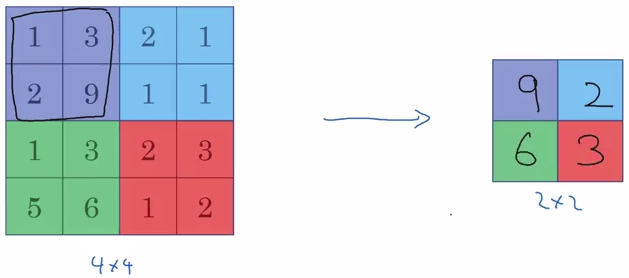
\includegraphics[width=0.8\textwidth]{max_pooling}
\caption{Max pooling with $f=2, s=2$.}
\label{fig:max_pooling}
\end{figure}

As noted above, the aim is to reduce the dimensionality while keeping the most important information about the input. The max pooling layer has two parameters: $f$ which is the size of the region considered, so here $f=2$. The stride $s$ is again the amount we move the region between each evaluation, so here $s=2$ as well. So if $s<f$, there will be overlap between the squares.

$s$ and $f$ are hyperparameters, i.e. they are not learnable - max pooling layers always remain the same during training.

That is the process for one channel. It is simply performed the same way for each channel. So a max pooling layer does not change the number of channels.

\subsubsection{Average pooling}
Another type of pooling layer - though it is infrequently used - is the \textit{average pooling} layer. It does exactly what you'd expect from the name: It works exactly the same as the max pooling layer, except is uses the mean value, not the maximum of pixel values.

\subsection{CNN structure with pooling layers}
A typical convolutional networks structure starts with a number of a number of layers - actually pairs of layers, but the terminology is common - consisting of a convolutional layer followed by a pooling layer. Then these are followed by a number of fully connected layers ending in a softmax output layer (for classification).

As we move through the convolution/pooling layers, usually the height and width of the "image" decreases, while the the number of channel increases.

\end{document}